\chapter*{Niveau 2}
\addcontentsline{toc}{chapter}{Niveau 2}
Du har lært at brygge de lidt mere avancerede drikke. Du kan se flere muligheder i mange af de urter du kender, og det er nu muligt for dig at påvirke spillet mere end før.\\
\begin{table}[H]
    \centering
    \begin{tabular}{|p{0.50\textwidth}|p{0.25\textwidth}|}
    \rowcolor{cerulean!80}\hline
        Evne navn & Pris i XP \\\hline
         Alkymi Niv. 2 & 2 \\\hline
         Læse/Skrive Magi & 1 \\\hline
         Personlig Have Niv. 1 & 2 \\
         \hline
    \end{tabular}
\end{table}
\section*{Evne beskrivelse}
\addcontentsline{toc}{section}{Evne beskrivelse}

\subsection*{Alkymi Niv. 2}
\addcontentsline{toc}{subsection}{Alkymi Niv. 2}
Du kan nu brygge en af de nedenstående drikke ud over de drikke du har adgang til i niveau 1. Alle disse drikke kræver specifikke ingredienser, og kun du kan blande dem korrekt.\\

\begin{table}[H]
    \centering
    \begin{tabular}{|c|c|}
        \rowcolor{cerulean!80}\hline
        Drik & Gift \\\hline
        Blodorkens styrke &  Den lærtes mund \\\hline
        Drømmeløs hvile & Ewens humør \\\hline
        Helbredelsesdrik & Smertedrik \\\hline
        Kranieforstærker & Svag Giftdrik\\\hline
        Stenhud &  Søvndrik\\\hline
        \multicolumn{2}{|c|}{Speciel} \\\hline
        \multicolumn{2}{|c|}{Velsignet Olie} \\\hline
    \end{tabular}
    \caption{Oversigt over niveau 2 drikke.}
\end{table}

\begin{drik*}[Blodorkens styrke]
\textbf{Type:} Positiv drik \\
\textbf{Ingredienser:} 1 Dværgerod \& blod fra en blodork.\\
\textbf{Indtagelse:} Drikkes\\
\textbf{Effekt:} Når du drikker denne drik, får du +4NK i 30 min.
\end{drik*}

\begin{gift*}[Den lærtes mund]
\textbf{Type:} Negativ drik\\
\textbf{Ingredienser:} 3 Ildgræs\\
\textbf{Indtagelse:} Drikkes / Blandes med væske / Evnen Påfør Gift\\
\textbf{Effekt:} Den som indtager denne gift skal sige alt hvad de tænker, i de næste 10 minutter.
\end{gift*}

\begin{drik*}[Drømmeløs hvile]
\textbf{Type:} Positiv Drik\\
\textbf{Ingredienser:} Blodbær \& Kongetand \& Tudsebark \\
\textbf{Indtagelse:} Drikkes\\
\textbf{Effekt:} Når denne drik indtages, falder spilleren i søvn i 10 min. Efter disse 10 min vil alle naturlige LP være genvundet, men vækkes spilleren inden 10 min er gået, vil drikken ikke have nogen effekt og spilleren genvinder ingen LP.\\
\end{drik*}

\begin{gift*}[Ewens humør]
\textbf{Type:} Negativ drik\\
\textbf{Ingredienser:} Tudsebark \& Ildgræs\\
\textbf{Indtagelse:} Drikkes / Blandes med væske\\
\textbf{Effekt:} Når du drikker denne drik, er du venner med alt og alle og har bare lyst til at snakke med alle. Denne drik vare i 30 minutters.
\end{gift*}

\begin{drik*}[Helbredelsesdrik]
\textbf{Type:} Øjeblikkelig Drik\\
\textbf{Ingredienser:} 2 Kongetand\\
\textbf{Indtagelse:} Drikkes\\
\textbf{Effekt:} Denne drik helbreder 2 LP. Du kan aldrig blive helbredt for mere end dit max LP.\\
\end{drik*}


\begin{drik*}[Kranieforstærker]
\textbf{Type:} Positiv Drik\\
\textbf{Ingredienser:} Ildgræs \& Jern\\
\textbf{Indtagelse:} Drikkes\\
\textbf{Effekt:} Når du drikker denne drik bliver du immun overfor evnen Bonk de næste 30 min.\\
\end{drik*}

\begin{drik*}[Præstindens tårer]
\textbf{Type:} Øjeblikkelig Drik\\
\textbf{Ingredienser:} Velsignet vand \& Ildgræs \& Tudsebark \& Kongetand.\\
\textbf{Indtagelse:} Drikkes\\
\textbf{Effekt:} Fjerner alle positive og negative effekter fra Drikke og Gifte.
\end{drik*}

\begin{gift*}[Smertedrik]
\textbf{Type:} Negativ Gift\\
\textbf{Ingredienser:} 2 Vorterod\\
\textbf{Indtagelse:} Drikkes / Blandes med væske / Evnen Påfør Gift\\
\textbf{Effekt:} Den som indtager denne drik vil blive påvirket af smerte. Hvilket er en effekt, hvor du bliver ramt af en ulidelig smerte. Du skal derfor skrige og spille på, at du har ubærlige smerter i 30 sekunder.\\
\end{gift*}

\begin{drik*}[Stenhud]
\textbf{Type:} Positiv Drik\\
\textbf{Ingredienser:} Blod \& Kvælertang\\
\textbf{Indtagelse:} Drikkes\\
\textbf{Effekt:} Denne drik giver dig 2 LP over dit maks LP, som ikke kan genvindes. Effekten aftager, når der er gået 30 min eller, når du har mistet de ekstra LP.\\
\end{drik*}


\begin{gift*}[Svag Giftdrik]
\textbf{Type:} Øjeblikkelig Gift\\
\textbf{Ingredienser:} Tudsebark \& Vorterod\\
\textbf{Indtagelse:} Drikkes / Blandes med væske / Evnen Påfør Gift\\
\textbf{Effekt:} Når du bliver forgiftet af denne drik, mister du 2 LP.\\
\end{gift*}

\begin{gift*}[Søvndrik]
\textbf{Type:} Negativ Gift\\
\textbf{Ingredienser:} 2 Kvælertang\\
\textbf{Indtagelse:} Drikkes / Blandes med væske / Evnen Påfør gift.\\
\textbf{Effekt:} Når du indtager denne drik, vil du falde i søvn og sove de næste 5 min.\\
\end{gift*}

\begin{særlig*}
\textbf{Type:} Særlig\\
\textbf{Ingredienser:} Velsignet vand, en helbredende drik, Blodbær.\\
\textbf{Indtagelse:} Smøres på en klinge.\\
\textbf{Effekt:} Klingen denne olie smøres på vil give helligskade de næste 30 minutter. Dette skal markeres med et grønt bånd.
\end{særlig*}

\subsection*{Læse/Skrive Magi}
\addcontentsline{toc}{subsection}{Læse/Skrive Magi}
Du kan læse og skrive skrift, der er skrevet på Magisk.\\
\begin{figure}[H]
    \centering
    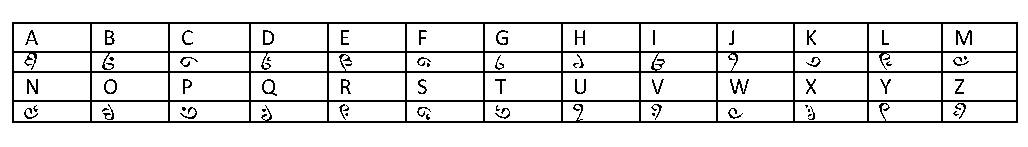
\includegraphics[width=1\textwidth]{setup/Alfabeter/Magisk alfabet.pdf}
    \caption{Magisk alfabet}
\end{figure}

\subsection*{Personlig Have Niv. 1}
\addcontentsline{toc}{subsection}{Personlig Have Niv. 1}
Som en del af din spilgang kan du vælge et område som skal være din have. Vi foreslår at dette område er afmærket så det er tydeligt.\\
I løbet af en spilgang kan du vælge at plante en urt i din have. Dette betyder at du mister en urt, men ved starten af næste spilgang vil du få 3 af denne urt tilbage.\\
Vi vil meget gerne opfordre spillere til at søge hjælp fra andre til at 'velsigne', 'luge' eller 'gøde' deres have så dette kan give godt spil.\\
\textit{\textbf{Eksempel:} Johannes har en have, hvor han planter Slangefrø. Han mister derfor den pose med Slangefrø, han har, og som en del af spillet søger han hjælp med en druide, og to krigere. Druiden velsigner jorden, mens krigerne hjælper ham med at fjerne ukrudt. Dette bliver godkendt af en arrangør, men han nævner det også ved næste indcheck. Derfor får han udleveret 5 Slangefrø, selvom han normalt kun ville blive givet 3.}
\\
